% DFF template for Latex and A4 paper.
% 12pt Times New Roman on 1.5 line spacing and 2 cm margins.

% ----------------------------------------------------------------------

% Either format with 
%    pdflatex projectdescription.tex
% Or if you use dvips and ps2pdf, remember to specify A4 paper:
%    latex  projectdescription
%    dvips  -ta4 projectdescription -o projectdescription.ps
%    ps2pdf -sPAPERSIZE=a4 projectdescription.ps

% ----------------------------------------------------------------------

\documentclass[fleqn,12pt]{article}
%Do not change this geometry settings
\usepackage[a4paper,top=2cm,bottom=2cm,left=2cm,right=2cm]{geometry}
\usepackage{times}
\usepackage[english]{babel}
\usepackage[utf8]{inputenc}
\usepackage[T1]{fontenc}
\usepackage[numbers,sort&compress]{natbib}
\usepackage[pdftex]{graphicx}
\usepackage{hyperref}
%\usepackage{titlesec}
\hypersetup{
    colorlinks=true,
    linkcolor = black,
    citecolor =blue,
    filecolor=magenta,      
    urlcolor=cyan,
}

% \usepackage{graphicx}         % For PDF figures
% \usepackage[dvips]{graphicx}  % For EPS figures, using dvips + ps2pdf

\begin{document}
% Empirically this seems to match MS Word's idea of 1.5 line spacing.
% DO NOT CHANGE
\setlength{\baselineskip}{1.44\baselineskip}


% ----------------------------------------------------------------------
% Enter the topic of the project and your names 

\begin{flushleft}
  {\large Gergo Gyori (gegy@itu.dk), BSc Data Science \\
  Katalin Literati-Dobos (klit@itu.dk), BSc Data Science \\
  Ludek Cizinsky (luci@itu.dk), BSc Data Science \\
  Lukas Rasocha (lukr@itu.dk), BSc Data Science \\}
 \end{flushleft}
 
\begin{center}
  {\Large Reflections on Data Science 2023}\\[5ex]
  {\Large Social Study: Herding effect on Reddit}\\[5ex]

 \end{center}
 

% ----------------------------------------------------------------------
% Delete the instruction 

%\parskip=3mm

%\noindent

\parindent=20pt 
\parskip=0mm

\section{Introduction}
Posts that achieve popularity on social media platforms, 
like Reddit, often outperform average posts significantly, 
which indicates a qualitative difference between popular posts 
and the rest. With this phenomenon an interesting question emerges:
is the success of a post attributable to its inherent quality,
or is it influenced by the herd effect? The social psychological 
behaviour that leads individuals to perceive an action as the 
appropriate course simply because it's what "everyone else" 
seems to be doing. This effect has already been documented in various studies such as \cite{muchnik} \cite{salganik}.
In this study we aim to investigate the herd effect on the Reddit platform, more
concretely, we want to find out to what extent does an initial upvote to a post
influence its future score?


\section{Experiment implementation}
Similar to Muchnik et al. \cite{muchnik}, to test the effect of a social
influence on upvoting reddit posts we conducted a randomised control trial.
For the continous period of seven days we collected and monitored recently published posts with no upvotes 
nor comments from the subreddit \textit{r/all}, and randomly assigned them 
to two categories: \textit{treatment} and \textit{control}.
The treatment group received an initial upvote, while the control group did not. 
The experiment was scheduled to run daily to ensure that the collected posts
had at least 24 hour period between the score loggings.

After the experimentation period ended, we aimed to test the following null hypothesis, with a significance
threshold $\alpha$ set to 0.05:
\textit{A treatment of a post does not influences its score (number of upvotes minus downvotes) in the future.}
Before the testing, some pre-processing steps were necessary. 
First, we removed the posts which were not continously monitored for a week and secondly,
to account for our initial upvote, we subtracted it from the posts' last day scores.
This resulted in a total number of $1578$ posts, i.e. $789$ treated posts and $789$ control posts. 
Finally, since we did not want to make assumptions about the underlying 
distribution of the data, we used non-parametric tests, namely Permutation test and Kolmogorov-Smirnov test, to
confirm or reject the studied null hypothesis.

\section{Results}
In this study we investigated the impact of initial positive
engagement on the future popularity of Reddit posts and whether 
such initial engagement can lead to a herd effect amongst users. 
Below we show the results of our experiment in terms of the scores of the posts
that are measured as a difference between the number of upvotes and downvotes.

The analysis began with the examination of basic summary statistics
of both the control and treatment groups with a focus
on the last day of the monitoring period for each post. Interestingly enough,
the mean score of the control group ($52.67$) was higher than of the treatment group ($35.51$),
which might suggest that the initial upvote had a negative effect on the future score of the posts.
However, it is important to note, that the standard deviation of both groups was very high, 
i.e. $417.63$ and $190.21$ for the control and treatment groups respectively, which indicates
that the scores of the posts were very spread out. So a few outliers that received a lot of upvotes
in the control group could have skewed the mean score upwards. This is furher supported by the median
which was $1$ for both groups.

Furthermore, these statistics only describe the distributions 
within each group. To determine whether there's a significant 
difference between the two groups, that is whether the 
initial upvote has a significant effect on the final score a post 
receives, we need to conduct other in depth statistical tests.
Since the skewness in the data could potentially violate assumptions
of some popular statistical tests, such as the t-test, we decided to use
non-parametric tests.

The null hypothesis
that the treatment has no effect on the future score of a post
could be tested by looking at the observed difference of the means of both groups
and then asking a question, how likely it is to observe such a difference
if the null hypothesis is true. If the probability of observing such a difference
is low (less than the significance threshold $\alpha$), then we can reject the null hypothesis.
Permutation test is a statistical technique that uses the collected data to create 
a distribution of the test statistic under the null hypothesis. Since
the observed difference is itself a random variable we can use this simulation
to estimate the distribution of mean differences under the null hypothesis from which the $p$-value can be infered. 
From $1000$ bootstrapped mean values in Figure \ref{fig:bootstrap_both_means} of both groups we can observe the groups' mean difference
and the larger spread in the control group. In order to test
whether our observed difference is significant we used Figure \ref{fig:mean_difference},
where $1000$ bootstrapped mean differences are plotted which have been randomly chosen 
by shuffling the concatenation of the last day scores from both groups. The observed difference is marked
with a red dashed line and the $p$-value can be calculated as the proportion of bootstrapped mean differences
that are greater or equal to the observed difference. The $p$-value is $0.325$ which is above
the significance threshold $\alpha = 0.05$ and thus the null hypothesis cannot be rejected.


\begin{figure}[h]
  \centering
  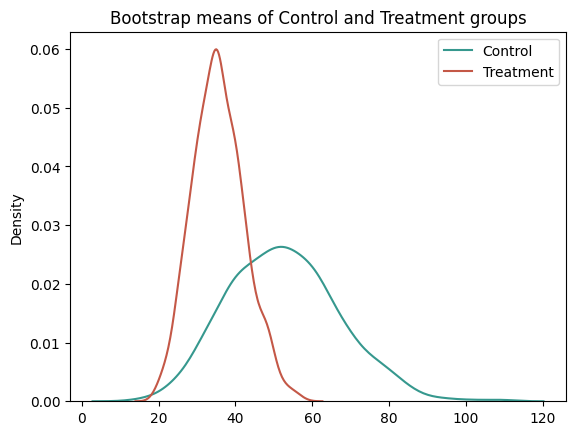
\includegraphics[width=0.4\textwidth]{figures/both_means.png}
  \caption{Bootstrapped means of control and treatment groups}
  \label{fig:bootstrap_both_means}
\end{figure}

\begin{figure}[h]
  \centering
  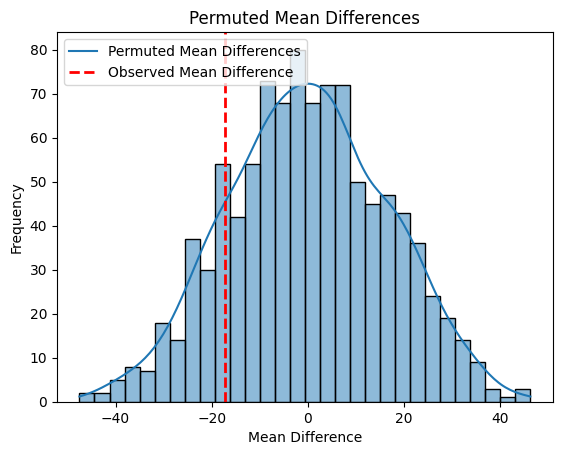
\includegraphics[width=0.4\textwidth]{figures/permutation_test.png}
  \caption{Permutation test of the mean differences between the control and treatment groups. The red dashed line indicates the observed difference.}
  \label{fig:mean_difference}
\end{figure}

Since the permutation test is looking at a single statistic (e.g. the mean difference)
it does not take into account the whole distribution of the data. For this
purpose we used the Kolmogorov-Smirnov (KS) test, which evaluates
whether the overall distributions of both groups are the same. 
The KS test showed a $p$-value of $6.77 \times 10^{-23}$ which indicates
that the control and treatment groups come from different distributions,
as their Empirical Cumulative Distribution Function (ECDF) significantly differ.
To further convince ourselves we plotted the ECDFs of both groups in Figure \ref{fig:ecdf}, which 
don't seem to differ much.
That is why we attempted to remove the low end of the scores (i.e. scores equal to or less than 1) which resulted in a $p$-value
of $0.17$ suggesting that the difference is primarily 
driven by the posts that have scores of 1 or less with no 
significant difference for the posts with the score of 2 or more.
This difference may thus be attributed to the randomness of vote fuzzing that will
be further discussed in the next section.

\begin{figure}[h]
  \centering
  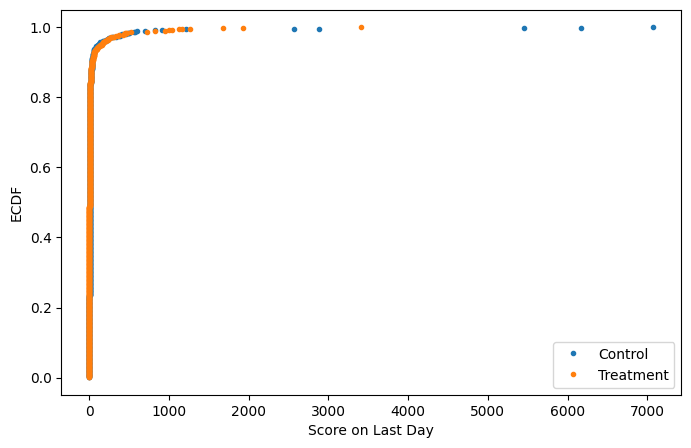
\includegraphics[width=0.5\textwidth]{figures/ecdf.png}
  \caption{ECDF of control and treatment groups}
  \label{fig:ecdf}
\end{figure}

To sumarise, according to our experiment and the data collected, one
could not confidently say that an initial upvote has any significant effect on the final 
score of a reddit post. This, together
with the experiment's limitations will be further discussed 
in the following section.

\section{Discussion}

The goal of our experimental design was to examine a null hypothesis
that a treatment has no effect on the future score of a post. To
test this hypothesis we employed a field experiment on the Reddit platform from which
we sampled new posts and randomly assigned them to our treatment and control groups.
This gave us the ability to assess the effect of our independent variable, the initial upvote,
on a quantifiable dependent variable, the future score of the post, while
still giving us some degree of control over the extraneous variables. 
This control stems from our sampling approach, by choosing
only recent posts that received no upvotes or comments and
the underlying premise of the randomisation approach which assumes
that with a sufficiently large sample size, the extraneous variables
will on average be equally distributed between both the groups, thus any
difference in the dependent variable could be attributed to the independent variable.
Nevertheless, due to the huge variability of posts on Reddit in terms
of content, length, time of posting and the diverse nature of the Reddit community,
we argue that our sample size of $1578$ posts might not be large enough to
fully remedy the potential confounding effects of the extraneous factors.

Another substantial limitation, which we discovered too late in the process,
was the vote fuzzing mechanism employed by Reddit to prevent vote manipulation. This mechanism
randomly adds or subtracts a small number of votes from the post's actual score, which in addition
is not visible to the user for some time after the post is submitted.
This makes it difficult to assess the true effect of the initial upvote
on the post's future score as the initial upvote might be offset back to $0$ and vice versa
the posts in the control group might appear with a random upvote/s. One possible way
we could have addressed this in our study would be to collect multiple measurements of the same post
and then average them out, but this would require a lot more computational time
and resources. Another way would be to collect other metrics of quality such as the number of comments
since they are not being altered with by the fuzzing mechanism.

Additionally, by choosing a very broad subreddit (r/all) we might have introduced 
moderating variables in terms of the diverse user bases that interact with the posts. 
These variables
could in turn influence the strength of the relationship between the independent
and dependent variable. Focusing on a more specific user base, such as
football fans or gamers, could have helped to control for this effect more effectively.
Another extraneous factor that might be present are intervening variables, a type of variables that are affected by the independent
variable and in turn affect the dependent variable.
For instance the reddit ranking algorithm might favour posts which were upvoted early on
and thus simply make them appear higher on the page. So the popularity of the post
could be attributed to the ranking algorithm rather than the herding effect. 



Our methods for statistical significance testing were also not without their limitations.
For instance the permutation approach operates under the assumption that our sampled data 
is a correct representation of the true population. If this assumption does not hold
then the results would be misleading.

Despite the limitations and complexities associated with this 
study, we hope that our experimental design and statistical 
analyses offer valuable insights into the role of initial positive reinforcement and social 
influence on post's popularity. For the sake of reproducibility, we also submit 
our experiment code and collected data as a part of this report.


\section{Conclusion}

In this study, a randomised field experiment was conducted to examine the effect of an 
initial upvote on the future score of a post on Reddit. After collecting and monitoring newly submitted posts
for a period of 7 days we conducted a statistical analysis with a Permutation test and a Kolmogorov-Smirnov test.
The results showed no significant indication that an initial upvote has any effect on the future score of a post.
However, due to the limitations such as the vote fuzzing mechanism, the results presented here should be interpreted with caution.


% ----------------------------------------------------------------------
% References 

 \newpage 
%\section*{References}
\bibliographystyle{unsrt}
\bibliography{yourbib}

\end{document}